% vim: set tw=78 sts=2 sw=2 ts=8 aw et:
\documentclass{so.cs.pub.ro}

\usepackage{code/highlight}

\title[Laborator 5]{Laborator 5}
\subtitle{Comunicare între Procese}
\date{21 - 27 Martie 2013}

\begin{document}

\frame{\titlepage}

% Titlul unui frame se specifică fie în acolade, imediat după \begin{frame},
% fie folosind \frametitle
\begin{frame}{Comunicare între procese}
        \begin{itemize}
        \item Procesele din cadrul unui sistem
        \begin{itemize}
        		\item pot fi independente
        		\item pot coopera / colabora
        \end{itemize}  
        		\vspace{0.3cm}
        \item Proces independent
        \begin{itemize}
        		\item nu afectează / nu este afectat de execuția altui proces 
        \end{itemize}
        		\vspace{0.3cm}
        \item Proces care colaborează
        \begin{itemize}
            \item poate afecta / fi afectat de execuția altui proces 
        		\item necesită mecanisme de comunicare între procese
        		\item avantaje
		      \begin{itemize}
        			\item partajare informații
        			\item speed-up computațional
        			\item modularitate
        		\end{itemize}        		
        \end{itemize}
      \end{itemize}
\end{frame}

\begin{frame}{Mecanisme IPC}
\begin{columns}
\begin{column}[1]{0.55\textwidth}
\framebox{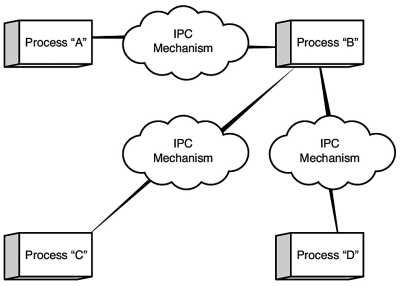
\includegraphics[width=2.5in]{code/IPC.jpg}}
\end{column}
\begin{column}[1]{0.35\textwidth}
      \begin{itemize}
        \item Ce mecanisme IPC cunoașteți?
      \end{itemize}
\end{column}
\end{columns}
\end{frame}

\begin{frame}{Mecanisme IPC}
      \begin{itemize}
        \item Semafoare 
        \begin{itemize}
        		\item modalitate de sincronizare
        \end{itemize}
        		\vspace{0.2cm}
        \item Cozi de mesaje / Mailslots
        \begin{itemize}
        		\item comunicarea are loc prin transfer de mesaje între procesele ce colaborează
        \end{itemize}  
        		\vspace{0.2cm}      
        \item Memorie partajată / FileMapping
        \begin{itemize}
        		\item se stabilește o zonă de memorie partajată de procesele ce cooperează
        		\item procesele pot schimba informații citind/scriind date din/în această zonă de memorie
        \end{itemize}
      \end{itemize}
\end{frame}

\begin{frame}{Semafoare POSIX}
  \begin{itemize}
		\item Named (sem_t)
  			\begin{itemize}
			 \item Identificare prin “/nume”, inter-proces
			 \item sem_open(), sem_close() sem_unlink()
		  \end{itemize}
		\item Unnamed (sem_t)
		  \begin{itemize}
			\item In general inter-thread pentru acelasi proces
			\item sem_init(), sem_destroy()
		  \end{itemize}
		\item P: sem_wait(), sem_trywait → EAGAIN ;)
		\item V: sem_post(), o unitate
		\item - implementare eficienta: futex(2) (Fast Userspace muTEX)
			\begin{itemize}
			 \item Evitare context-switch-uri pe anumite cazuri (care?)
			\end{itemize}
		\item Linux: prezente ca /dev/shm/sem.nume  
  \end{itemize}
\end{frame}

\begin{frame}{Cozi de mesaje POSIX}
  \begin{itemize}
		\item Man 7 mq_overview
		\item Identificare prin „/nume”, tip mqd_t (intreg)
		\vspace{0.3cm}		
		\item mq_open
		\vspace{0.3cm}
		\item mq_send - len $<=$ msgsize
		  \begin{itemize}
			\item msgsize  - dimensiunea maximă permisă pentru un mesaj
		  \end{itemize}
		\item mq_receive - len $>=$ msgsize
		\vspace{0.3cm}		
		\item mq_close / mq_unlink
		\vspace{0.3cm}		
		\item Linux, maximul implicit: /proc/sys/kernel/msgmax
		\item Debug: mount -t mqueue none /my/path
  \end{itemize}
\end{frame}

\begin{frame}{Memorie partajata(Linux)}
  \begin{itemize}
		\item Man 7 mq_overview
		\vspace{0.3cm}
		\item shm_open
		\vspace{0.3cm}
		\item ftruncate
		  \begin{itemize}
		\item Inițial, zona de memorie are dimensiune zero
		  \end{itemize}
		\vspace{0.3cm}
		\item mmap
		\item munmap
		\vspace{0.3cm}
		\item close
		\item shm_unlink
  \end{itemize}
\end{frame}

\begin{frame}{API Windows}
\begin{columns}
\begin{column}[1]{0.43\textwidth}
  \begin{itemize}
		\item Semafoare
	   \begin{itemize}
			\item CreateSemaphore
			\item OpenSemaphore
			\item WaitForSingleObject
			\item ReleaseSemaphore
			\item CloseHandle
  		\end{itemize}
		\vspace{0.1cm}  
  		\item Cozi de mesaje
  		\begin{itemize}
			\begin{beamerboxesrounded}[lower=block body,shadow=true]{}
      		\small{\centerline {\textbackslash\textbackslash.\textbackslash mailslot\textbackslash [path]$<$nume$>$}}
			\end{beamerboxesrounded}
			\vspace{0.1cm}  
			\item CreateMailslot
			\item CreateFile 
			\item ReadFile
			\item WriteFile
			\item CloseHandle
 		\end{itemize}
  \end{itemize}
\end{column}
\begin{column}[1]{0.57\textwidth}
      \begin{itemize}
      	\item Memorie partajată
  			\begin{itemize}
				\item CreateFileMapping
				\item OpenFileMapping
				\item MapViewOfFile
				\item UnmapViewOfFile
				\item CloseHandle
  			\end{itemize}        
      \end{itemize}
\end{column}
\end{columns}
\end{frame}

%\begin{frame}{Întrebări}
%\begin{itemize}
%\item Procesele P1 și P2 au fiecare câte un pointer către o zonă de memorie partajată ce conține șirul "AB".
%Ce va conține zona de memorie după ce fiecare din procese execută: \newline 
%for(i = 0; i \textless 2; i++) p[i]++;
%\item Există vreo diferență între un mutex și un semafor binar?
%\item Într-un sistem de planificare bazat pe priorități dați exemplu de o situație în care un task cu prioritate mare
%poate fi împiedicat să ruleze
%pentru că sistemul este ocupat să ruleze un task cu prioritate mică.
%\end{itemize}
%\end{frame}

\end{document}
